\begin{comment}
\title{parslTestbookQMCblog}
\author{Dr. Sou-Cheng Choi, Illinois Tech and SouLab, Joshua Jay Herman (QMC Development Team)}
\date{September 2025}

\maketitle
Accelerating QMCpy Notebook Tests with Parsl
\end{comment}

\subsection{Introduction}

 This blog post summarizes the speedup of notebook regression testing presented in our talk at ParslFest 2025 \cite{parslfest2025} 
 and highlights subsequent directions of the work. Regression testing of notebooks for QMCPy \cite{QMCPy2020a} is massively parallel and resource-intensive. The slides can be found at \href{https://github.com/QMCSoftware/QMCSoftware/raw/refs/heads/parsl_presentation/demos/talk_paper_demos/Parslfest_2025/Parsl%20Testbook%20Speedup.pptx}{Parsl Testbook Speedup}

\subsection{Methodology}

 Choosing Testbook \cite{testbook2021} is motivated by the ability of writing a test that can execute the notebook itself and it also fits well with our tests in a separate directory, where we have already implemented other tests without requiring execution of the full notebooks for clarity. We made a test harness that we could also have Parsl \cite{parsl2019} execute our testbook unit tests since it is embarrassingly parallel problem..

\subsection{Results}

To determine a baseline speedup with a subset of notebooks, we observed a speedup. 
After expanding our test coverage to search for syntax errors in additional notebooks, we now see a 4.4-fold speedup, which is consistent with our expectations, as illustrated in Figure~\ref{fig:parsl_speedup}. 

\begin{figure}[htbp]
    \centering
    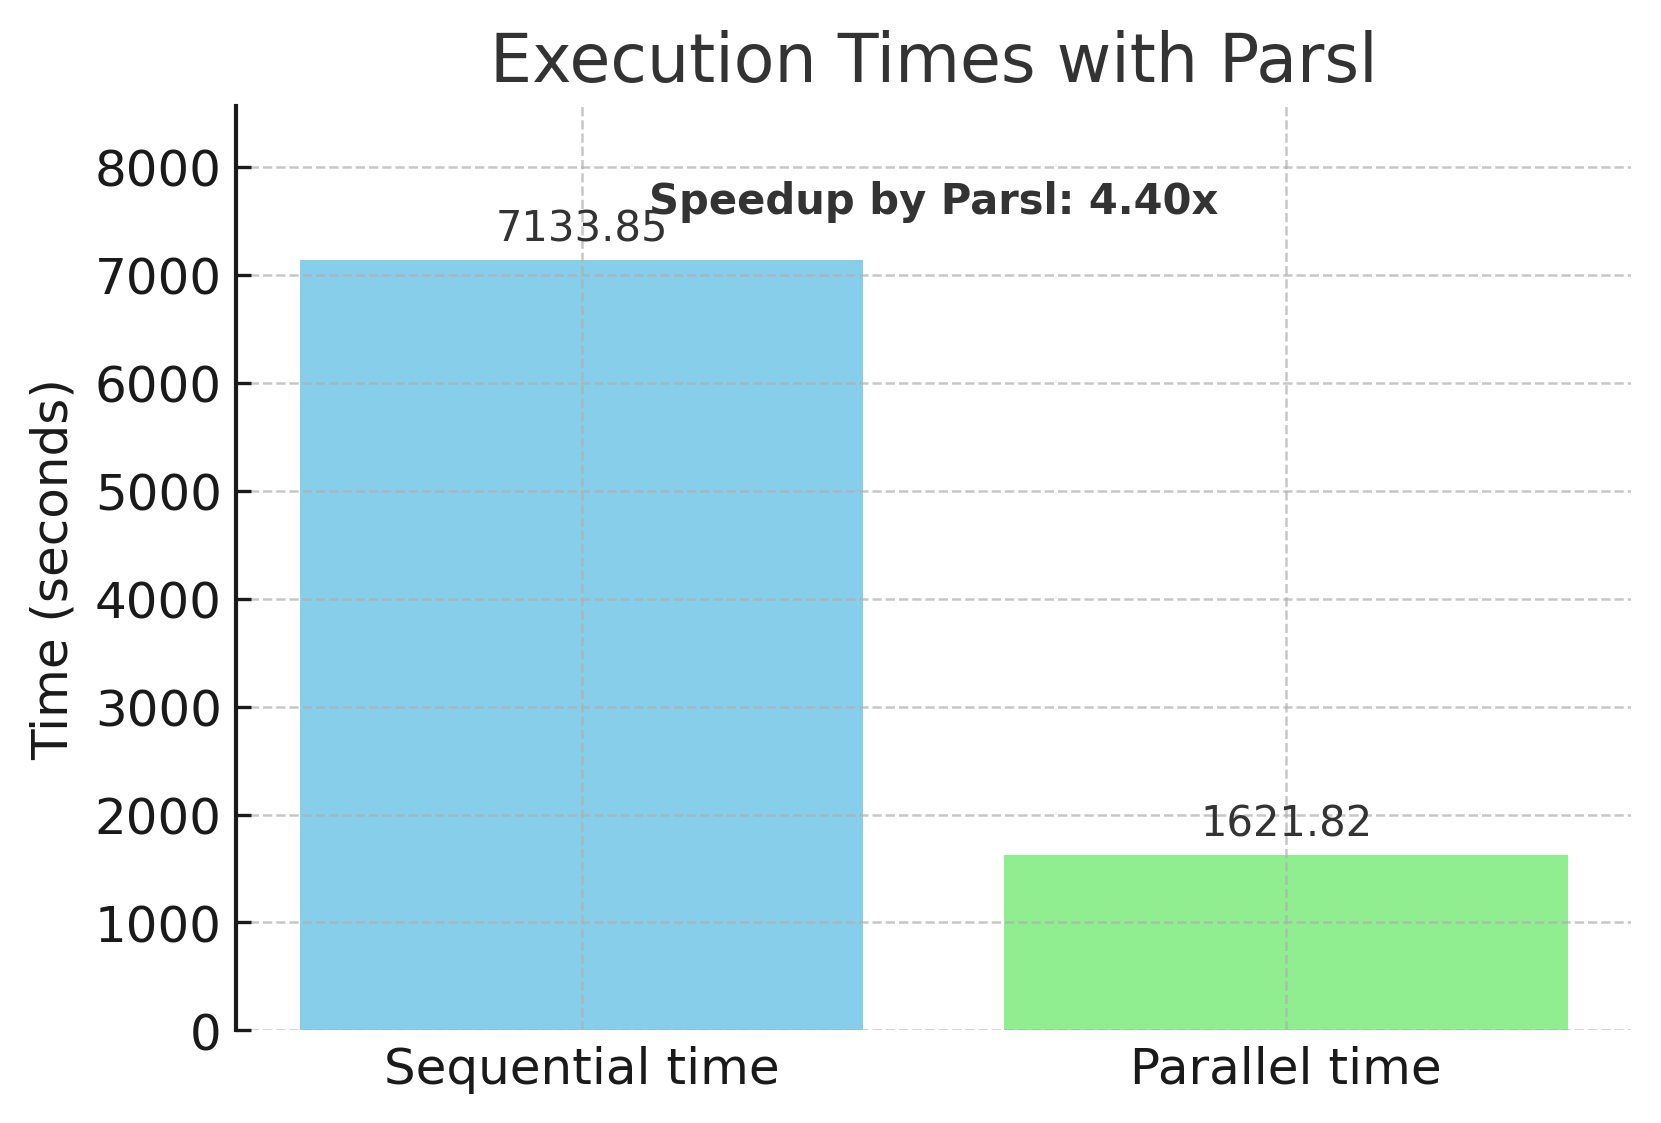
\includegraphics[width=.7\textwidth]{booktests/parsl_speedup_chart_no_x_lines.png}
    \caption{Parallel testing speedup using Parsl against sequential execution of tests.}
    \label{fig:parsl_speedup}
\end{figure}

This was tested on a Linux system running on an AMD64 architecture with 16 CPU cores. If you want to run the tests we have made for QMCPy you can run 'make testbook'

\subsection{Further Work}

Due to the above results, this indicates that we should extend our testing to doctest and pytests in Parsl.

Now, because many people have multi‑core processors, we can increase individual productivity so that our tests can demonstrate that no regressions have been introduced.

Furthermore, regarding feedback on the presentation to the ParslFest participants, the system is quite general. This suggests a distributed test system could benefit Parsl users by enabling them to distribute their own test workloads.

Finally, we could expand our work to encompass Python doctests, as well as unit testing using pytest or unittest, in addition to testing Jupyter notebooks.